% \chapter{植被冠层和土壤水分}
%\addcontentsline{toc}{chapter}{陆地表面的水分循环}

\chapter{植被冠层水分}\label{植被冠层截留}

% \section{植被冠层截留}\label{植被冠层截留}
\begin{mymdframed}{代码}
本章对应的代码文件为\texttt{MOD\_LeafInterception.F90}。
\end{mymdframed}

冠层是降水的首要接触层,它对降水的再分配有着重要的作用。CoLM冠层的水量平衡方程基本与SiB2一致~\citep{sellers1996revised},主要基于以下控制方程:
\begin{equation}\label{eq:冠层水量控制方程}
\frac{\partial M_{cw,s}}{\partial t} = P-D_{d}-D_{c}-E_{ci} / \rho_{w}
\end{equation}
式中$P$为总降水量(\unit{m.s^{-1}}),分为对流降水和大尺度降水类型:
\begin{equation}\label{eq:降水类型}
P=P_{c}+P_{l}=\left(R_{c}+S_{c}\right)+\left(R_{ls}+S_{ls}\right)
\end{equation}
其中下标$c$和$ls$代表对流和大尺度降水类型,$R$和$S$分别代表降雨率与降雪率(\unit{m.s^{-1}})。当驱动强迫场中只有总降水可用时,CoLM假设大尺度降水等于$1/3P$,对流降水占$2/3P$。
$D_d$为降雨穿透速率(\unit{m.s^{-1}}),即从冠层间隙下落的降水速率,$D_c$为冠层排水速度(\unit{m.s^{-1}}),$\frac{\partial M_{cw,s}}{\partial t}$为冠层蓄水变化率(\unit{m.s^{-1}}),$\rho_w$是水的密度,$E_{ci}$为蒸发速率。

CoLM支持包括CoLM2014、CLM4.5、CLM5.0、VIC、MATSIRO、JULES 和Noah-MP等多种冠层截留计算参数化方案。具体的区别如表~\ref{tab:不同截留方案比较} 所示。
%
%\begin{table}[htbp]
%\caption{不同截留方案的比较}
%\label{tab:不同截留方案比较}
%\begin{center}
%\begin{tabular}{p{2cm}{c}p{1.5cm}{c}p{1.5cm}p{1.5cm}p{1.5cm}p{1.5cm}p{1.5cm}p{1.5cm}p{1.5cm}{c}}
%\toprule
%模式 & 叶倾角 & 独立的雨雪过程 & 雪的卸载 & 叶片水的相变 & 可变最大冠层水深 & 降水的形态和网格分布 & 独立叶温计算 & 重力排水\\\midrule
%CoLM2014 & 是 & 否 & 否 & 否 & 否 & 是 & 否 & 否 \\
%CLM4.5 & 否 & 否 & 否 & 否 & 否 & 否 & 否 & 否 \\
%CLM5 & 否 & 是 & 是 & 否 & 否 & 否 & 否 & 否 \\
%Noah-Mp & 否 & 是 & 否 & 是 & 是 & 是 & 是 & 否 \\
%VIC & 否 & 是 & 否 & 是 & 是 & 是 & 是 & 否 \\
%MATSIRO & 否 & 是 & 否 & 是 & 是 & 是 & 否 & 是 \\
%JULES & 否 & 是 & 否 & 是 & 是 & 是 & 否 & 是 \\
%\bottomrule
%\end{tabular}
%\end{center}
%\end{table}

\begin{table}[htbp]
\centering \renewcommand{\arraystretch}{1.5}
\caption{不同截留方案的比较}
\label{tab:不同截留方案比较}
\begin{tabular}{p{2cm}ccccccc}
\toprule
模式 & CoLM2014 & CLM4.5 & CLM5 & Noah-MP & VIC & MATSIRO & JULES \\\midrule
叶倾角 & \checkmark & $\times$ & $\times$ & $\times$ & $\times$ & $\times$ & $\times$ \\
独立的雨雪过程 & $\times$ & $\times$ & \checkmark & \checkmark & \checkmark & \checkmark & \checkmark \\
雪的卸载 & $\times$ & $\times$ & \checkmark & $\times$ & $\times$ & $\times$ & $\times$ \\
叶片水的相变 & $\times$ & $\times$ & $\times$ & \checkmark & \checkmark & \checkmark & \checkmark \\
可变最大冠层水深 & $\times$ & $\times$ & $\times$ & \checkmark & \checkmark & \checkmark & \checkmark \\
降水的形态和网格分布 & \checkmark & $\times$ & $\times$ & \checkmark & \checkmark & \checkmark & \checkmark \\
独立叶温计算 & $\times$ & $\times$ & $\times$ & \checkmark & \checkmark & $\times$ & $\times$ \\
重力排水 & $\times$ & $\times$ & $\times$ & $\times$ & $\times$ & \checkmark & \checkmark \\
\bottomrule
\end{tabular}
\end{table}
以下针对不同方案分别进行详细介绍。

\section{CoLM2014方案}
在CoLM2014方案中,公式~\eqref{eq:冠层水量控制方程} 中的直接穿透量$D_d$与辐射传输中的光穿透量的计算方法一致,由下式给出:
\begin{equation}
D_{d}=\delta_{P} \cdot P=\delta_{P} \cdot\left(R_{c}+S_{c}+R_{l}+S_{l s}\right)
\end{equation}
其中$\delta_P$是冠层穿透系数,等于
\begin{equation}
\delta_{P}=1.0-\alpha \times\left[1-\exp \left(-K_{p} \times LSAI\right)\right]
\end{equation}
该公式中反映叶片集水能力的经验系数$\alpha$被设定为0.25~\citep{lawrence2011parameterization}。
$LSAI$是$SAI$和$LAI$之和($LAI$和$SAI$分别是叶指数和茎面积指数);$K_p$是消光系数,与辐射在冠层中的穿透计算相同:
\begin{equation}\label{eq:消光系数}
\begin{aligned}
K_{p} &= \phi_{1}+\phi_{2} \\
\phi_{2} &= 0.877\left(1-2 \phi_{1}\right) \\
\phi_{1} &= 0.5-0.633 \chi_{L}-0.33 \chi_{L}^{2}
\end{aligned}
\end{equation}
$K_p$通过叶角分布的经验参数$\chi_L$的变化来控制,其中$\chi_L=0$表示球形叶角分布,$\chi_L= 1$表示水平方向的叶子,$\chi_L= -1$表示垂直方向的叶子。根据植被类型,$\chi_L$的范围在$-0.3\sim0.25$之间。由此计算得出的$\delta_P$的变动范围如图~\ref{fig:穿透系数与叶面积指数} 所示。
{
\begin{figure}[htbp]
\centering
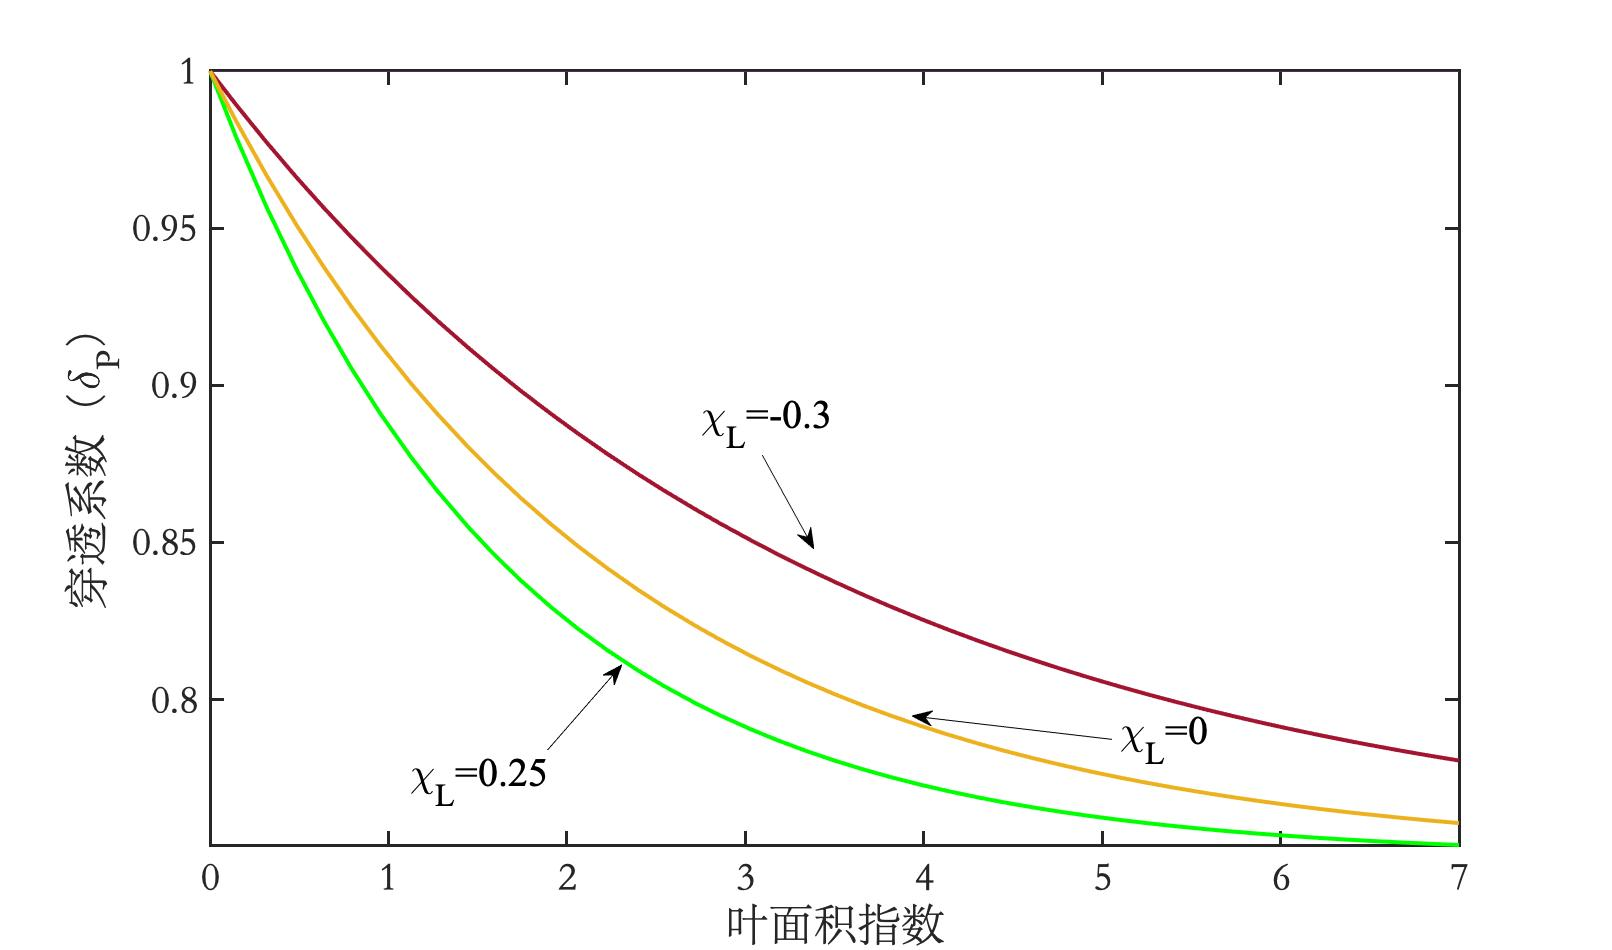
\includegraphics[width=1.0\textwidth]{Figures/陆地表面的水分循环/穿透系数与叶面积指数.jpg}
\caption{穿透系数$\delta_P$与叶面积指数的关系及其变动范围}
\label{fig:穿透系数与叶面积指数}
\end{figure}
}

为防止升华或冷凝水超过最大树冠储存量,CoLM在计算冠层截留之前首先更新树叶上的水深($L_{dew}$) (mm):
\begin{equation}
\begin{aligned}
L_{dew} &= L_{dew}-x_{sc} \\
x_{s c} &= \max\left(0., L_{dew}-S_{c}\right)
\end{aligned}
\end{equation}
其中$x_{sc}$是超过最大树冠储存量的水(mm),$S_c=0.1\left(LAI+SAI\right)$代表最大蓄水量(mm)。
$x_{sc}$的相位首先由冠层温度决定。如果冠层温度大于冰点温度,CoLM假定所有过量的水都处于液相,否则处于冰雪相。
{
\begin{figure}[htbp]
\centering
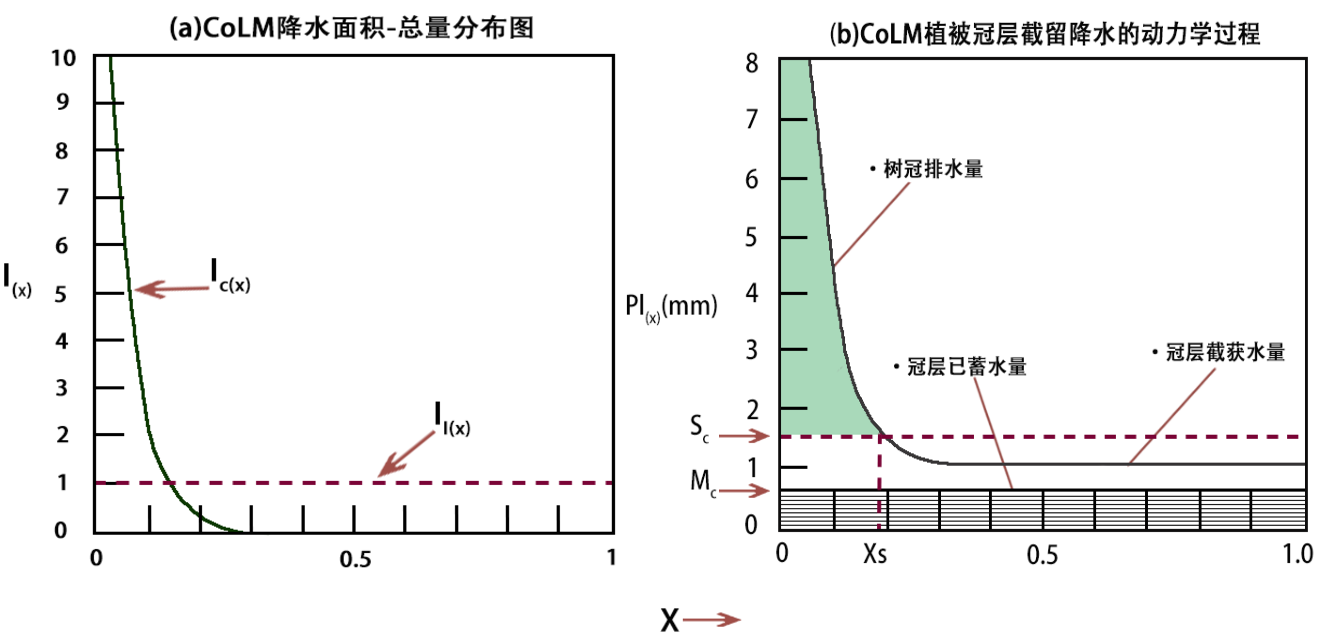
\includegraphics[scale=0.6]{Figures/植被冠层和土壤水分/CoLM冠层截留示意图.pdf}
\caption[(a) CoLM中使用的降水面积-总量分布图;(b) CoLM中植被冠层截留降水的动力学过程]{(a) CoLM中使用的降水面积-总量分布图(修改自SiB2)。其中变量$x$为网格面积的比例,变量$I_{\left(x\right)}$为相对降水量。值得注意的是,大尺度降水$I_l\left(x\right)$在网格区几乎是不变的,而对流降水$I_c\left(x\right)$是非均匀分布的;(b) CoLM中植被冠层截留降水的动力学过程。降雨截留前已储存在冠层中的水量$M_{cs}-M_{cw}$被假设是均匀分布在网格区域上的。$M_{cs}-M_{cw}$的以上的水量积分即为冠层截获的总水量。$xs$是网格区域拦截降雨的比例加上先前存在的树冠蓄水($M_{cs}-M_{cw}$)所超过了树冠最大储水量($S_c$)的水量。所有大于$S_c$的水量假设形成树干径流,而低于$S_c$的水量则被保存在冠层之中}
\label{fig:CoLM冠层截留示意图}
\end{figure}
}

如图~\ref{fig:CoLM冠层截留示意图}a 所示,CoLM假设网格内的降水的分布是不均匀的。其中对流降水面积的网格占比$I_c$可以由下式给出
\begin{equation}
I_{c}(x)=a_{c} e^{-bx}+c_{c}
\end{equation}
其中$a_c=20$,$b=20$和$c_c=0.206\times10^{-8}$是常数。大尺度降水面积的网格占比$I_l$可以用相同的形式表示:
\begin{equation}
I_{l}(x)=a_{l} e^{-b x}+c_{l}
\end{equation}
其中$a_l=0.0001$和$c_l=0.9999$。因此,通过组合这两个方程给出了有效降水占比区域的降雨强度为:
\begin{equation}
P I(x)=\left(a_{l} P_{l}+a_{c} P_{c}\right) e^{-b x}+\left(c_{l} P_{l}+c_{c} P_{c}\right)
\end{equation}
如图~\ref{fig:CoLM冠层截留示意图}b 所示,因此,有效降水区域的树冠排水($thru_{rain}$)由下式给出:
\begin{equation}
thru_{rain}=\int_{0}^{x_{s}} P I(x) d x+L_{dew} x_{s}-S_{c} x_{s}
\end{equation}
其中$x_s$是单位网格中截获降水加上原有冠层蓄水量超过冠层上允许的最大水深($S_c$)的比例:
\begin{equation}
x_{s}=\frac{-1}{b} \log \left[\frac{s_{c}-L_{d e w}}{a_{p}\left(P-D_{d}\right)}-\frac{c_{p}}{a_{p}}\right]
\end{equation}
即树冠截取的雨量等于或者超过其饱和极限网格面积的比例。其中$a_p=\frac{a_lP_l+a_cP_c}{P}$,$c_p=\frac{c_lP_l+c_cP_c}{P}$。这里假设只有液态水能够被从冠层落下,我们有
\begin{equation}
thru_{rain}=\left(R_{c}+R_{l}\right)\left(1-\delta_{p}\right) \frac{a_{p}}{b}\left(1-e^{-b x_{s}}\right)+c_{p} x_{s}+L_{dew} x_{s}-S_{c} x_{s}
\end{equation}
在整体网格尺度上$D_c$被更新为
\begin{equation}
D_c=thru_{r a i n}+x_{s c}
\end{equation}
因此,保留在树冠上的可用于树冠蒸发(截留蒸发)的蓄水量$L_{dew}$ (mm)可以由下式进行更新:
\begin{equation}
L_{dew}={P}-D_{c}-D_{d}
\end{equation}
在冠层蒸发量的计算上首先需要计算湿叶茎面积占总叶茎面积的比例 ($f_{wet}$)。该计算CoLM模型采用~\citet{dickinson1993biosphere}提出的经验方法
\begin{equation}
f_{{wet}}=\left(\frac{L_{dew, p}}{s_{c}}\right)^{2 / 3} \leqslant 1.0
\end{equation}
其中$L_{dew, p}$是上一步计算得出的可用于树冠蒸发的蓄水量 (m)。因此,树冠蒸发量计算如下:
\begin{equation}
E_{ci} / \rho_{w}=\min \left(\frac{\left(q_{s}-q_{sat}^{T_{c}}\right)}{r_{b} /\left(LSAI \times f_{wet}\right)}, \frac{L_{dew}}{\Delta t}\right)
\end{equation}
这里$r_b$是平均边界层阻力,由冠层顶部的风速和特征叶片尺寸确定;$q_{sat}^{T_c}$ (\unit{kg kg^{-1}})是冠层温度下的饱和比湿度;$q_s$为表层参考高度处的比湿度,$\Delta t$为时间步长。


\section{CLM4.5方案}
CLM4.5的冠层截留方案~\citet{oleson2013technical}~和CoLM2014的方案非常类似。主要的区别在于公式~\eqref{eq:消光系数} 中的$K_p$的计算。
$K_p$在CLM4.5冠层截留方案中取固定值0.5,即:
%
\begin{equation}
\delta_{P}=1.0-\alpha \times\left[1-\exp \left(-0.5 \times LSAI\right)\right]
\end{equation}
则直接穿透量由下式给出:
\begin{equation}
D_{d}=\delta_{P} \cdot P=\delta_{P} \cdot\left(R_{c}+S_{c}+R_{l}+S_{l s}\right)
\end{equation}

为了保持模型构架的一致性,我们和CoLM一样在计算冠层截留之前首先更新树叶上的水深 ($L_{dew}$) (mm):
\begin{equation}
\begin{aligned}
L_{dew} &= L_{dew}-x_{sc} \\
x_{s c} &= \max \left(0., L_{dew}-S_{c}\right)
\end{aligned}
\end{equation}
请注意在原生CLM4.5方案中没有这一步骤。

由于CLM4.5方案中并不考虑网格内部的降水类型和分布(假设降水均匀分布在整个网格上),则降水区域的冠层排水$thru$:
\begin{equation}
thru=P\left(1-\delta_{p}\right)+L_{dew}-S_{c}
\end{equation}
在整体网格尺度上$D_c$被更新为
\begin{equation}
D_c=thru+x_{s c}
\end{equation}
其他均与CoLM2014方案保持一致。

\section{CLM5.0方案}
CLM5.0的参数化方案与CLM4.5有较大的差别~\citep{lawrence2019community}。其中最重要的差别之一是对雨和雪的截留方案的进一步细化,但不考虑网格内部的降水类型和分布。在CLM5中,液态水的降落过程和CoLM、CLM4.5类似。液态降水在通过冠层时要么被树冠截留,要么直接落到雪/土壤表面(穿透)或从植被上滴下(树冠滴流)。固态降水的处理也类似,额外考虑先前截留的雪的卸载(unloading)。具体计算流程如下:

\begin{enumerate}
\item 分别计算固态和液态水在叶片上的最大蓄水量(mm):
\begin{equation}
S_{c,rain}=0.1(LAI+SAI)
\end{equation}
\begin{equation}
S_{c,snow}=6.0(LAI+SAI)
\end{equation}
\item 分别计算固态和液态降水的直接穿透速率:
\begin{equation}
\delta_{P,rain}=1.0 - \alpha_{rain} \tanh(LAI+SAI)
\end{equation}
\begin{equation}
\delta_{P,snow}=1.0 - \alpha_{snow}\left\{1-\exp\left[-0.5(LAI+SAI)\right]\right\}
\end{equation}
这里$\alpha_{rain}$和$\alpha_{snow}$的值与CLM4.5、CoLM的$\alpha$ (0.25)不同,在CLM5中被设定为1.0。穿透速率也被拆分为:
\begin{equation}
D_{d,rain}=\delta_{P,rain}(R_c+R_{ls})
\end{equation}
\begin{equation}
D_{d,snow}=\delta_{P,snow}(S_c+S_{ls})
\end{equation}
\item 计算冠层排水速率:
\begin{equation}
thru_{rain}=(R_c+R_{ls})(1-\delta_{p,rain})+L_{dew,rain}-S_{c,rain}
\end{equation}
\begin{equation}
thru_{snow}=(S_c+S_{ls})(1-\delta_{p,rain})+L_{dew,snow}-S_{c,snow}
\end{equation}
CLM5额外考虑了冠层积雪的卸载速率:
\begin{equation}\label{q_unl_wind}
q_{unl,wind}=\frac{uL_{dew,snow}}{1.56\times 10^5}
\end{equation}
\begin{equation}
q_{unl,temp}=\max\left[0, \frac{L_{dew,snow}(T-270)}{1.87\times 10^5}\right]
\end{equation}
\begin{equation}\label{q_unl_tot}
q_{unl,tot}=\min(q_{unl,wind}+q_{unl,temp},L_{dew,snow})
\end{equation}
固态和液态的排水速率为:
\begin{equation}
D_{c,rain}=thru_{rain}
\end{equation}
\begin{equation}
D_{c,snow}=thru_{snow}+q_{unl,tot}
\end{equation}
\end{enumerate}
其他参数计算均参照CoLM2014方案。


\section{Noah-MP方案}
Noah-MP模型冠层截留方案的计算流程与CoLM2014、CLM4.5和CLM5有较大的区别~\citep{niu2011community,he2023modernizing}。具体介绍如下:
\begin{enumerate}
\item 分别计算理想状态下固态和液态水在叶片上的最大蓄水量(mm)\\
\begin{equation}
S_{c,rain}=0.1\left(LAI+SAI\right)\\
\end{equation}
\begin{equation}
S_{c,snow}= 6.6\left(0.27+{\frac{46}{\rho_{s}}}\right) \left(LAI+SAI\right)
\end{equation}
其中$\rho_{s}$是降雪堆积密度: 
\begin{equation}
\rho_{s}=67.92+51.25 e^{\frac{T_{sfc}-T_{frz}}{2.59}}
\end{equation}

\item 计算冠层闭郁度$F_{veg}$:
\begin{equation}
F_{veg} = \max\left[0.05,1.0-e^{-0.52\left(LAI+SAI\right)}\right]
\end{equation}
\item 分别计算固态和液态降水直接穿透速率:
\begin{equation}
D_{d,rain}=\left(1.0-F_{veg}\right) \times (R_{c}+R_{ls})
\end{equation}
\begin{equation}
D_{d,snow}=\left(1.0-F_{veg}\right) \times (S_{c}+S_{ls})
\end{equation}
\item 如有积雪,则考虑其积雪的卸载,该方案与CLM5所用的方案完全一致(公式~\eqref{q_unl_wind}--\eqref{q_unl_tot})。
\item 计算当前冠层水的相态变化:
\begin{enumerate}
\item 冠层固态水转变为液态水,如果表面温度高于0度:
\begin{equation}
\begin{aligned}
q_{can, melt} &=\min \left(\frac{L_{dew,snow}}{\Delta t},\ \left(T_{v}-T_{frz}\right) \times \frac{C_{ice} \times L_{dew,snow}}{\rho_{i c e} \times C_{LH, fus} \times \Delta t}\right) \\ 
L_{dew,snow} &=\max \left(0.0,\ L_{dew,snow}-q_{c a n, m e l t} \times \Delta t\right) \\
L_{dew,rain} &=\max \left(0.0,\ L_{dew,rain}-L_{dew,snow}\right)
\end{aligned}
\end{equation}
\item 冠层液态水转变为固态水,如果表面温度低于0度:
\begin{equation}
\begin{aligned}
q_{c a n, f r z} &=\min \left(\frac{L_{dew,rain}}{\Delta t},\ \left(T_{f r z}-T_{v}\right) \times \frac{C_{wat} \times L_{dew,rain}}{\rho_{wat} \times C_{LH, fus} \times \Delta t}\right) \\ 
L_{dew,rain} &=\max \left(0.0,\ L_{dew,rain}-q_{can, frz} \times \Delta t\right) \\
L_{dew,snow} &=\max \left(0.0,\ L_{dew,snow}-L_{dew,rain}\right)
\end{aligned}
\end{equation}
\end {enumerate}
其中$q_{can, melt}$是固态转换为液态的速率(融化速率),$q_{can, frz}$是液态转换为固态的速率(凝结速率),$T_{v}$为空气温度(K),$T_{frz}$是相态变化温度(273.15 K),$C_{ice}$是冰的比热容(\unit{J.m^{-3}.K^{-1}}),$C_{wat}$是液态水的比热容(\unit{J.m^{-3}.K^{-1}}),$\Delta t$是时间步长(s),$C_{LH, fus}$是融合潜热(\unit{J.kg^{-1}}),$\rho_{ice}$是冰的密度(917 \unit{kg.m^{-3}}),$\rho_{wat}$是水的密度(1000 \unit{kg.m^{-3}})。这一步的主要目的是更新$L_{dew,rain}$和$L_{dew,snow}$。

\item 如有降水发生,则计算当前降雨条件和闭郁度情况下接触冠层的最大水量(interception capability):
\begin{equation}
Q_{intr,rain} =F_{veg}\left(R_{c}+R_{ls}\right)\times FP
\end{equation}
\begin{equation}
Q_{intr,snow} =F_{veg}\left(S_{c}+S_{ls}\right)\times FP
\end{equation}
假设对流降水在网格中是不均匀分布的,则$FP$(网格中降水发生的比率)计算如下:
\begin{equation}
FP = P/ (10P_{c} + P_{ls})
\end{equation}
\item 计算当前时刻降水被拦截且被保留的实际网格水量:
\begin{equation}
Q_{intr,rain} = \min\left[Q_{intr,rain}, \ \frac{(S_{c,rain} - L_{dew,rain})}{\Delta{t}}  (1-e^{-\left(R_{c}+R_{ls}\right)\Delta{t}/S_{c,rain}})\right]
\end{equation}
\begin{equation}
Q_{intr,snow} = \min\left[Q_{intr,snow},\ \frac{(S_{c,snow} - L_{dew,snow})}{\Delta{t}} (1-e^{-\left(S_{c}+S_{ls}\right)\Delta{t}/S_{c,snow}})\right]
\end{equation}
其中${\Delta{t}}$是计算时间步长。
\item 更新当前冠层固态和液态的排水速率,以及冠层的对应水深
\begin{equation}
D_{c,rain}=F_{veg} \times (R_{c}+R_{ls})-Q_{intr,rain}
\end{equation}
\begin{equation}
D_{c,snow}=F_{veg} \times (S_{c}+S_{ls})-Q_{intr,snow}
\end{equation}
\end{enumerate}
其他计算均参照CoLM2014方案。


\section{VIC方案}
VIC的冠层截留方案~\citep{liang1994simple,hamman2018variable}主要基于~\citet{storck2002measurement}在俄勒冈一个山区气候站点的积雪积累和消融观测结果。
\begin{enumerate}
\item 分别计算固态和液态水在叶片上的最大蓄水量(mm)\\
首先计算雨加上雪的总最大拦截容量为:
\begin{equation}
I_{max} = 4.0 m (LAI+SAI)
\end{equation}
其中$m=0.5$ mm 是根据最大雪拦截容量观测结果确定。
除了对水总量的储水能力有限制之外,模式还分别对固态和液态水在叶片上的最大蓄水量进行了限制:
\begin{equation}
S_{c,rain}=0.1\left(LAI+SAI\right)+0.035 L_{dew,snow}\\
\end{equation}
\begin{equation}
S_{c,snow}=L_r m (LAI+SAI)
\end{equation}
其中$L_r$是温度的函数:
\begin{equation}
L_r = \begin{cases}
           4.0, & T_a > -1 \text{ \textcelsius}\\
            1.5, & -3 \text{ \textcelsius} < T_a \leqslant -1 \text{ \textcelsius}\\
           1.0, & T_a \leqslant -3 \text{ \textcelsius}
         \end{cases}
\end{equation}
这基于前人的被拦截雪观测结果以及该场站的数据~\citep{storck2002measurement}。\citet{kobayashi1987snow}~观察到随着气温降低到 $-3$ \textcelsius 以下,较窄表面上的最大雪拦截负荷急剧下降。 \citet{kobayashi1987snow}和~\citet{pfister1999snow}的观测结果表明,当温度低于 $-1$ \textcelsius 时,拦截效率显著下降,当温度低于 $-3$ \textcelsius 时大致恒定,因此导致函数的不连续。

\item 计算冠层闭郁度$F_{veg}$
\begin{equation}
F_{veg} = \max\left[0.0,\ (LAI+SAI)\right]
\end{equation}

\item 分别计算固态和液态降水直接穿透速率:
\begin{equation}
D_{d,rain}=\left(1.0-F_{veg}\right) \times (R_{c}+R_{ls})
\end{equation}
\begin{equation}
D_{d,snow}=\left(1.0-F_{veg}\right) \times (S_{c}+S_{ls})
\end{equation}

\item 计算当前冠层水的相态变化,更新$L_{dew,snow}$ 和 $L_{dew,rain}$,这一部分的方案和Noah-MP一致。

\item 当发生降水,如果降水的形态是固态,且温度小于 $-3$ \textcelsius ,风速大于1 \unit{m.s^{-1}},则当前时刻冠层积雪的卸载由风速和冠层雪水当量共同决定:
\begin{equation}
D_{d,snow} = \min\left[L_{dew,snow},\ (0.2u-0.2) \times L_{dew,snow}\right]
\end{equation}

\item 冠层排水速率的计算
\begin{equation}
thru_{rain}=\left(R_{c}+R_{ls}\right)\left(1-\delta_{p,rain}\right)+L_{dew,rain}-S_{c,rain}
\end{equation}
\begin{equation}
thru_{snow}=\left(S_{c}+S_{ls}\right)\left(1-\delta_{p,snow}\right)+L_{dew,snow}-S_{c,snow}+D_{d,snow}
\end{equation}

\item 如更新排水计算后所得的截留的雨水和积雪的总量($L_{dew,rain}+L_{dew,snow}$)超过了树木的最大承载能力($I_{max}$),则需要将最大承载能力按固液比例进行卸载:
\begin{equation}
L_{dew,overload}=(L_{dew,rain}+L_{dew,snow}-I_{max})
\end{equation}
\begin{equation}
L_{dew,rain}=L_{dew,rain} - L_{dew,overload} \times \frac{L_{dew,rain}}{L_{dew,rain}+L_{dew,snow}}
\end{equation}
\begin{equation}
L_{dew,snow}=L_{dew,snow} - L_{dew,overload} \times   \frac{L_{dew,snow}}{L_{dew,rain}+L_{dew,snow}}
\end{equation}
\begin{equation}
thru_{rain}=thru_{rain} + \frac{L_{dew,rain}}{L_{dew,rain}+L_{dew,snow}}
\end{equation}
\begin{equation}
thru_{snow}=thru_{snow} + \frac{L_{dew,snow}}{L_{dew,rain}+L_{dew,snow}}
\end{equation}
\end{enumerate}
其他计算均参照CoLM2014方案。


\section{MATSIRO方案}
MATSIRO的冠层截留方案主要基于~\cite{storck2002measurement}在俄勒冈一个山区气候站点的积雪积累和消融观测结果。
\begin{enumerate}
\item 分别计算固态和液态水在叶片上的最大蓄水量(mm)\\
\begin{equation}
S_{c,rain}=0.2\left(LAI+SAI\right)
\end{equation}
\begin{equation}
S_{c,snow}=0.2\left(LAI+SAI\right)
\end{equation}

\item 计算冠层闭郁度$F_{veg}$
\begin{equation}
F_{veg} = \max\left[0, \left(LAI+SAI\right)\right]
\end{equation}

\item 分别计算固态和液态降水直接穿透速率:
\begin{equation}
D_{d,rain}=\left(1.0-F_{veg}\right) \times (R_{c}+R_{ls})
\end{equation}
\begin{equation}
D_{d,snow}=\left(1.0-F_{veg}\right) \times (S_{c}+S_{ls})
\end{equation}
\item 计算当前冠层水的相态变化,方案和Noah-MP一致。

\item 当降水发生时,将网格拆分成强对流区域(Storm area)和大尺度降水区域(Non-Storm area)。其中对流降水面积的比例假设为均匀状态(0.1),而大尺度降水面积的比例则假设为1。则在强对流区域,固态和液态水在叶片上的蓄水量为:
\begin{equation}
L_{dew,rain,s}=L_{dew,rain}+(F_{veg}R_{ls}+F_{veg}R_{c}/0.1)\times \Delta{t}
\end{equation}
\begin{equation}
L_{dew,snow,s}=L_{dew,snow}+(F_{veg}S_{ls}+F_{veg}S_{c}/0.1)\times \Delta{t}
\end{equation}
冠层排水速率的计算同时考虑了超过冠层容水量导致的滴水和重力导致的自然滴水:
\begin{equation}
thru_{rain,s}=L_{dew,rain,s}-S_{c,rain}+D_{1} \exp \left(D_{2} S_{c,rain}/1000\right)
\end{equation}
\begin{equation}
thru_{snow,s}=L_{dew,rain,s}-S_{c,snow}+D_{1} \exp \left(D_{2} S_{c,snow}/1000\right)
\end{equation}
下标$s$代表对流降水,$D_{1}=1.14 \times 10^{-11}$,$D_{2}=3.7 \times 10^{3}$。在计算完冠层排水之后,再次更新强对流区域的冠层水量。

\item 而在大尺度降水区域,固态和液态水在叶片上的蓄水量则为:
\begin{equation}
L_{dew,rain,n}=L_{dew,rain}+F_{veg}R_{ls}\times \Delta{t}
\end{equation}
\begin{equation}
L_{dew,snow,n}=L_{dew,snow}+F_{veg}S_{ls} \times \Delta{t}
\end{equation}
下标$n$分别代表强对流和大尺度降水.
同样冠层排水速率的计算同时考虑了超过冠层容水量导致的滴水和重力导致的自然滴水:
\begin{equation}
thru_{rain,n}=L_{dew,rain,n}-S_{c,rain}+D_{1} \exp \left(D_{2} S_{c,rain}/1000\right)
\end{equation}
\begin{equation}
thru_{snow,n}=L_{dew,rain,n}-S_{c,snow}+D_{1} \exp \left(D_{2} S_{c,snow}/1000\right)
\end{equation}
在计算完冠层排水之后,再次更新强大尺度区域的冠层水量。

\item 由于在拆分强对流和大尺度降水区域计算过程中,网格区域有所重叠(在计算强对流区域截留时同时考虑了大尺度降水),需要进一步进行加权平均得到网格平均:
%
\begin{equation}
\begin{aligned}
L_{dew,rain} & = L_{dew,rain,n} + (L_{dew,rain,s} - L_{dew,rain,n}) \times 0.1 \\
L_{dew,snow} & = L_{dew,snow,n} + (L_{dew,snow,s} - L_{dew,snow,n}) \times 0.1
%\end{equation}
%
%\begin{equation}
\end{aligned}
\end{equation}
%
在整体网格尺度上$D_c$亦被更新。

\end{enumerate}

\section{JULES方案}
JULES的参数化方案与CLM5.0方案较为接近。对雨和雪的截留方案的进一步细化,但不考虑网格内部的降水类型和分布。
\begin{enumerate}
\item 分别计算固态和液态水在叶片上的最大蓄水量(mm)\\
\begin{equation}
S_{c,rain}=0.1\left(LAI+SAI\right)\\
\end{equation}
\begin{equation}
S_{c,snow}=4.4\left(LAI+SAI\right)
\end{equation}
\item 计算冠层闭郁度$F_{veg}$
\begin{equation}
F_{veg} = \max\left[0.0,\left(LAI+SAI\right)\right]
\end{equation}

\item 计算当前冠层水的相态变化,方案和Noah-MP一致。

\item 当有降水发生时,分别计算固态和液态降水直接穿透速率:
\begin{equation}
D_{d,rain}=\left(1.0-F_{veg}\right) \times (R_{c}+R_{ls})
\end{equation}
\begin{equation}
D_{d,snow}=\left(1.0-F_{veg}\right) \times (S_{c}+S_{ls})
\end{equation}
\item 计算当前时刻降水被拦截且被保留的实际网格水量的方法与Noah-MP类似,不同点在于在额外增加了一个拦截效率系数$k(=0.6)$:
\begin{equation}
Q_{intr,rain} = \min\left[Q_{intr,rain},\,  k \times \frac{(S_{c,rain} - L_{dew,rain})}{\delta{t}} \left(1-e^{-\left(R_{c}+R_{ls}\right)\delta{t}/S_{c,rain}}\right)\right]
\end{equation}
\begin{equation}
Q_{intr,snow} = \min\left[Q_{intr,snow},\, k \times \frac{(S_{c,snow} - L_{dew,snow})}{\delta{t}}\left(1-e^{-\left(S_{c}+S_{ls}\right)\delta{t}/S_{c,snow}}\right)\right]
\end{equation}
其中${\delta{t}}$是计算时间步长。
\item 更新当前冠层固态和液态的排水速率,以及冠层的对应水深
\begin{equation}
D_{d,rain}=F_{veg} \times (R_{c}+R_{ls})-Q_{intr,rain}
\end{equation}
\begin{equation}
D_{d,snow}=F_{veg} \times (S_{c}+S_{ls})-Q_{intr,snow}
\end{equation}
\item 冠层排水速率的计算
\begin{equation}
D_{c,rain}=\left(R_{c}+R_{ls}\right)\left(1-\delta_{p,rain}\right)+L_{dew,rain}-S_{c,rain}
\end{equation}
\begin{equation}
D_{c,snow}=\left(S_{c}+S_{ls}\right)\left(1-\delta_{p,rain}\right)+L_{dew,snow}-S_{c,snow}
\end{equation}

\end{enumerate}






